% Compilación desde esta carpeta: tectonic paper.tex
% Alternativa con TeX Live/MiKTeX: pdflatex paper; bibtex paper;
% pdflatex paper; pdflatex paper. Requiere paquetes LaTeX estándar.
% IEEEtran.cls y IEEEtran.bst se distribuyen sin cambios bajo sus licencias.
% Regeneración opcional (no necesaria para compilar este ZIP):
% python generate_resources.py --results RUTA_RESULTADOS --output RUTA_FUENTE
% RUTA_RESULTADOS es results/ del paquete de código; RUTA_FUENTE recibe
% validation_rows.tex, ablation_rows.tex y figuras/{curves.pdf,confusion.pdf,error.jpg}.
% Dependencias: numpy==2.5.2, pandas==3.1.0, matplotlib==3.11.2.
% El CSV de confusión incluye las clases; no se requiere otra lista ni el dataset.
\def\encodingdefault{T1}
\documentclass[conference]{IEEEtran}
\usepackage[T1]{fontenc}
\usepackage{iftex}
\ifPDFTeX\usepackage[utf8]{inputenc}\fi
\usepackage[spanish,es-tabla,es-nodecimaldot]{babel}
\usepackage{amsmath,amssymb}
\usepackage{graphicx,booktabs,array}
\usepackage{cite}
\usepackage{tikz}
\usetikzlibrary{arrows.meta,positioning,babel}
\PassOptionsToPackage{hyphens,spaces}{url}
\usepackage[hidelinks]{hyperref}
\urlstyle{same}
\renewcommand{\IEEEkeywordsname}{Palabras clave}
\addto\captionsspanish{\renewcommand{\abstractname}{Resumen}}
\newcommand{\artifact}[1]{\texttt{\small #1}}
\begin{document}
\title{Reconocimiento de 40 platos peruanos con transferencia de aprendizaje: ResNet-18 frente a YOLO26m-cls}
\author{\IEEEauthorblockN{Josué Chilón Cruzado, Miguel Ángel Concepción Tiza, Enzo Israel Neyra Dianderas,\\
Omar Salvador Tello Guerra y Alexander Vladimir Paco Cornejo}
\IEEEauthorblockA{Grupo 3, MIA-203 Redes Neuronales y Aprendizaje Profundo\\
Maestría en Inteligencia Artificial, Universidad Nacional de Ingeniería\\
Lima, Perú, 2026}}
\maketitle
\begin{abstract}
Reconocer platos peruanos en fotografías permite organizar información gastronómica, pero una clasificación equivocada puede alterar la consulta posterior de ingredientes de una receta. Este trabajo compara ResNet-18 y YOLO26m-cls mediante transferencia de aprendizaje sobre PeruFoodNet, con 4.000 fotografías de 40 clases. Se adaptó la última capa lineal a 40 salidas y se contrastaron dos regímenes: entrenar únicamente esa capa o ajustar toda la red, con 10 y 40 imágenes por clase. La campaña incluyó 32 corridas: búsqueda de dos tasas con semilla 42 y repetición de las ocho condiciones seleccionadas con semillas 43 y 44. La elección utilizó exclusivamente F1 macro de validación. Con 40 imágenes por clase, YOLO26m-cls completo obtuvo 0,8903 $\pm$ 0,0076, frente a 0,8810 $\pm$ 0,0103 de ResNet-18 completo y 0,6990 $\pm$ 0,0049 de la línea base ResNet-18 de capa final. El checkpoint prefijado de semilla 42 alcanzó exactitud 0,9050 y F1 macro 0,9043 en 600 imágenes de prueba. Se analizaron confusiones y un error que modifica la ficha documental de ingredientes. Los resultados favorecen el ajuste completo dentro del espacio ensayado; la diferencia entre arquitecturas no demuestra superioridad estadística. La partición secuencial puede distribuir tomas de una misma ración entre conjuntos, por lo que las conclusiones se limitan a este protocolo y no acreditan generalización externa ni detección visual de alérgenos.
\end{abstract}
\begin{IEEEkeywords}
clasificación de alimentos, redes convolucionales, transferencia de aprendizaje, PeruFoodNet, análisis de errores
\end{IEEEkeywords}

\section{Introducción}
La diversidad de presentaciones de un plato dificulta su reconocimiento automático. En el contexto peruano, una fotografía puede servir como entrada para proponer un nombre y consultar información gastronómica. PeruFoodNet ofrece imágenes etiquetadas de platos tradicionales y listas de posibles ingredientes alergénicos por receta \cite{arzola2025}. El problema abordado es de \emph{clasificación monoclase}: dada una imagen, asignar una de 40 etiquetas. La ficha posterior depende del nombre propuesto; no se supervisa la presencia de ingredientes en la imagen.

Las redes neuronales convolucionales (CNN) aprenden filtros compartidos para extraer patrones espaciales y combinar representaciones visuales. Reutilizar pesos preentrenados reduce la necesidad de aprender todas esas representaciones desde pocos ejemplos. Se comparan ResNet-18, cuya estructura residual facilita la optimización \cite{he2016}, y la variante de clasificación YOLO26m-cls \cite{jocher2026}. ResNet-18 constituye una referencia consolidada; YOLO26m-cls permite estudiar una familia reciente bajo el mismo protocolo. Ambas producen 40 logits mediante una capa lineal adaptada. La pregunta es cómo cambian el F1 de validación y los errores al modificar la familia, el alcance del ajuste y el presupuesto de imágenes.

El aporte es experimental y de aplicación: se adaptan clasificadores existentes y se realiza una comparación propia, sin proponer un nuevo bloque neuronal. Las contribuciones verificables son:
\begin{enumerate}
\item Una comparación de dos familias, dos regímenes y dos presupuestos con selección por validación y tres semillas en las condiciones seleccionadas.
\item Una ablación de capa final frente a ajuste completo a tasa fija, separada de la comparación con tasas seleccionadas.
\item Un análisis reproducible de errores de prueba y de su efecto sobre una ficha de receta, con trazabilidad y límites de uso explícitos.
\end{enumerate}
La Sección II sitúa los antecedentes; la III describe el método; la IV presenta resultados, errores y costo; la V discute su alcance; y la VI concluye.

\section{Trabajos relacionados}
\subsection{Reconocimiento de comida y contexto peruano}
Food-101 estudia el reconocimiento de platos mediante componentes discriminativos y bosques aleatorios, y aporta un conjunto de referencia para este dominio \cite{bossard2014}. Ese trabajo evidencia que la comida puede abordarse como una tarea de reconocimiento visual; sus clases y su protocolo difieren de los nuestros, por lo que no se comparan directamente sus métricas. Arzola Gutierrez, Canchari Muñoz y Escobedo Cárdenas publicaron PeruFoodNet y relacionaron sus platos con ingredientes potencialmente alergénicos \cite{arzola2025}. Usamos su versión 3 \cite{perufoodnetv3}, sin atribuir al grupo la creación del dataset ni de sus recetas. El aporte propio es la matriz de transferencia y el análisis de la propagación de un error de clasificación a la consulta documental.

\subsection{Representaciones transferidas y optimización}
He et al. introdujeron el aprendizaje residual para facilitar el entrenamiento de redes profundas \cite{he2016}. Yosinski et al. estudiaron la transferencia y la especialización de características entre tareas \cite{yosinski2014}; esto motiva contrastar un extractor fijo con uno adaptable. El trabajo de YOLO26 presenta una familia unificada con variantes para varias tareas, incluida clasificación \cite{jocher2026}. Aquí se utiliza exclusivamente el clasificador, sin cajas, localización ni métricas de detección. Las innovaciones de su entrenamiento original no se atribuyen al bucle propio: este usa AdamW y entropía cruzada para ambas familias. AdamW desacopla el decaimiento de pesos de la actualización adaptativa \cite{loshchilov2019}; mantenerlo común evita introducir un optimizador diferente por arquitectura.

\subsection{Puntuación y uso responsable}
Guo et al. mostraron que las puntuaciones de redes modernas pueden estar mal calibradas \cite{guo2017}. Por ello, el máximo softmax se trata como puntuación operativa y no como probabilidad calibrada de acierto. El umbral aplicado en este proyecto no constituye un detector validado de imágenes ajenas al dominio. Tampoco existe un experimento de detección de ingredientes: la información asociada al plato procede de las tablas del dataset \cite{arzola2025}.

\section{Metodología}
\subsection{Datos, particiones y preprocesamiento}
PeruFoodNet V3 contiene 4.000 JPG, 40 platos y 100 fotografías por clase, y se distribuye bajo CC BY 4.0 \cite{perufoodnetv3}. El artículo describe capturas con distintas presentaciones, ángulos y condiciones \cite{arzola2025}. La licencia del dataset se distingue de la del artículo que lo documenta. Se conservaron todas las clases, sin curación de clases ni agrupación de vistas. El orden de etiquetas se fija en \artifact{data/classes.json}; el manifiesto mantiene rutas relativas, índices, números y particiones.

La Tabla~\ref{tab:data} resume el reparto solicitado según el número inicial del \emph{archivo} dentro de cada clase. Los presupuestos son anidados: 01--10 está incluido en 01--40. Las imágenes elegibles restantes de entrenamiento no se usaron. Validación selecciona tasas, épocas y configuración; prueba caracteriza únicamente el checkpoint fijado. La separación de archivos no acredita separación de raciones: fotografías correlacionadas pueden cruzar conjuntos e inflar las métricas. No se dispone de identificación de ración para comprobar independencia.

\begin{table}[t]
\caption{Partición por número de archivo en cada clase.}
\label{tab:data}\centering\small
\begin{tabular}{lrrr}\toprule
Uso & Números & Por clase & Total\\\midrule
Entrenamiento elegible & 01--70 & 70 & 2.800\\
Presupuesto reducido & 01--10 & 10 & 400\\
Presupuesto ampliado & 01--40 & 40 & 1.600\\
Prueba & 71--85 & 15 & 600\\
Validación & 86--100 & 15 & 600\\\bottomrule
\end{tabular}
\end{table}

Cada imagen se convierte a RGB y se redimensiona directamente a $224\times224$, sin recorte que preserve la proporción. Se aplica volteo horizontal aleatorio únicamente al entrenar. En la campaña se habilita caché de imágenes redimensionadas en RAM: la lectura inicial usa interpolación bilineal y el aumento se aplica después. Los canales se convierten a valores en $[0,1]$. ResNet emplea además media $(0{,}485,0{,}456,0{,}406)$ y desviación $(0{,}229,0{,}224,0{,}225)$ de ImageNet; YOLO mantiene la escala $[0,1]$. La geometría es comparable, mientras la normalización respeta cada familia. La evaluación no usa aumentos aleatorios.

\subsection{Arquitecturas y transferencia}
La Fig.~\ref{fig:architecture} representa el flujo. Los pesos locales iniciales son ResNet-18 ImageNet-1K V1 y YOLO26m-cls. Se reemplaza únicamente la última capa lineal de cada clasificador. Para un lote de $B$ imágenes, el extractor produce $h_\phi(x)\in\mathbb{R}^{B\times d}$ y la capa adaptada produce $z\in\mathbb{R}^{B\times40}$; $d$ depende de la familia. Cada logit corresponde a una clase en el orden del manifiesto.

En \emph{capa final} se optimizan solo los pesos y sesgos de la última capa lineal; los parámetros del extractor y las estadísticas de BatchNorm permanecen fijos. En \emph{red completa} se ajusta toda la red. Por tanto, ``cabeza'' no significa desbloquear todos los bloques que la biblioteca agrupa en su módulo de clasificación. Las comprobaciones del código contrastan parámetros congelados y estadísticas al terminar. Un adaptador común devuelve logits también cuando la implementación de YOLO retorna una tupla durante evaluación.

\begin{figure}[t]\centering
\begin{tikzpicture}[node distance=3.8mm,>=Stealth,
box/.style={draw,rounded corners=1pt,align=center,text width=7.4cm,minimum height=7mm,font=\footnotesize}]
\node[box] (input) {Fotografía RGB $\rightarrow$ redimensionamiento y normalización\\Entrada: $B\times3\times224\times224$};
\node[box,below=of input] (encoder) {Extractor preentrenado: ResNet-18 o YOLO26m-cls\\Representación agrupada: $B\times d$};
\node[box,below=of encoder] (linear) {Última capa lineal adaptada $d\rightarrow40$\\Logits: $B\times40$};
\node[box,below=of linear] (output) {Softmax $\rightarrow$ clase propuesta y puntuación máxima\\Marca incierta si puntuación $<0{,}50$};
\node[box,below=of output] (recipe) {Consulta documental por nombre de plato\\Ficha de receta; no detección visual de ingredientes};
\draw[->] (input)--(encoder);\draw[->] (encoder)--(linear);
\draw[->] (linear)--(output);\draw[->] (output)--(recipe);
\end{tikzpicture}
\caption{Flujo común. En capa final solo se ajusta la capa $d\rightarrow40$; en ajuste completo también se adapta el extractor. La consulta de receta queda fuera del modelo aprendido.}
\label{fig:architecture}
\end{figure}

\subsection{Pérdida, predicción y métricas}
Para una imagen $x_i$, la representación $h_\phi(x_i)$ y los parámetros lineales $(W,b)$ definen
\begin{equation}
z_i=Wh_\phi(x_i)+b,\quad
p_{ic}=\frac{\exp(z_{ic})}{\sum_{k=1}^{40}\exp(z_{ik})}.
\label{eq:logits}
\end{equation}
Con etiqueta $y_i\in\{1,\ldots,40\}$, la entropía cruzada media de un lote de tamaño $B$ es
\begin{equation}
\mathcal{L}_{\mathrm{CE}}=-\frac{1}{B}\sum_{i=1}^{B}\log p_{i,y_i}.
\label{eq:loss}
\end{equation}
Se entrega $z_i$ directamente a la función de entropía cruzada; no se aplica softmax antes de calcular la pérdida. No se incorporan pesos por clase ni suavizado de etiquetas. AdamW añade decaimiento desacoplado de pesos, distinto de introducirlo como término de la pérdida de la Ec.~\eqref{eq:loss}.

La predicción es $\hat y_i=\arg\max_c z_{ic}$. Con $N$ imágenes y conteos por clase $TP_c$, $FP_c$ y $FN_c$, se calculan
\begin{align}
\mathrm{Exactitud}&=\frac{1}{N}\sum_{i=1}^{N}\mathbf{I}(\hat y_i=y_i),\\
P_c&=\frac{TP_c}{TP_c+FP_c},\quad R_c=\frac{TP_c}{TP_c+FN_c},\\
F_{1,c}&=\frac{2TP_c}{2TP_c+FP_c+FN_c},\\
F_1^{\mathrm{macro}}&=\frac{1}{40}\sum_{c=1}^{40}F_{1,c}.
\end{align}
La indicadora $\mathbf{I}$ vale 1 cuando la predicción coincide con la etiqueta y 0 en caso contrario. Se consideran las 40 etiquetas y se asigna cero ante un denominador nulo. F1 macro da el mismo peso a cada plato y expone fallos específicos incluso con soportes equilibrados. La exactitud complementa el recuento global. La puntuación $s_i=\max_c p_{ic}$ marca incertidumbre si $s_i<0{,}50$; esas imágenes permanecen en todas las métricas.

\subsection{Entrenamiento y regla de selección}
El protocolo común usa AdamW, decaimiento de pesos $0{,}01$, lote 16 y tasas constantes $10^{-4}$ o $3\times10^{-4}$. No hay scheduler. La regularización compartida incluye decaimiento, volteo y parada temprana. Se fijan las semillas de Python, NumPy, PyTorch y el generador del cargador; se desactiva el benchmark de cuDNN y se activa su modo determinista. Esto documenta las condiciones locales sin garantizar identidad numérica en cualquier hardware.

El techo es 200 épocas por corrida, con paciencia 10 sin mejora \emph{estricta} del mejor F1 macro de validación. Un empate cuenta como una época sin mejora y conserva el primer máximo. Se evalúan entrenamiento y validación después de cada época con transformaciones deterministas. La pérdida de entrenamiento registrada es la evaluación posterior de todo su subconjunto, no la media de pérdidas de los lotes aumentados usados en las actualizaciones.

Primero se ejecutan $2\times2\times2\times2=16$ combinaciones con semilla 42. Para cada familia, régimen y presupuesto se escoge la tasa por F1 de validación; un empate exacto favorece la menor. Después se repiten \emph{solo esas ocho tasas} con semillas 43 y 44: otras 16 corridas, 32 en total. Las ocho condiciones se resumen con media y desviación \emph{muestral} de sus tres mejores F1:
\begin{equation}
\bar F=\frac{1}{3}\sum_{s=42}^{44}F_s,\qquad
\sigma_F=\sqrt{\frac{\sum_{s=42}^{44}(F_s-\bar F)^2}{3-1}}.
\end{equation}
La dispersión mide variación entre semillas sobre la misma partición, no incertidumbre sobre nuevas raciones. La tasa está seleccionada con semilla 42, lo que también condiciona esa estimación.

El ganador maximiza $\bar F$ únicamente entre configuraciones con 40 fotos por clase. El desempate exacto usa menor latencia medida en el mismo equipo; no fue necesario para el máximo observado. Se fijan la configuración y el checkpoint de \emph{semilla 42}, sin elegir la mejor semilla. Solo entonces se habilita prueba. Las comprobaciones de una época y la exploración preliminar de 15 épocas quedan fuera de la matriz final y de la selección.

\subsection{Implementación y trazabilidad}
El código separa preparación, carga, modelos, entrenamiento, experimentos, evaluación e inferencia. La campaña se ejecutó en Windows con RTX 5090 de aproximadamente 32 GB, PyTorch 2.11.0, torchvision 0.26.0 y Ultralytics 8.4.202. MLflow 3.18.0 se usa para seguimiento clásico de experimentos: una corrida padre, corridas hijas, metadatos de datasets de entrada, cinco métricas por época, configuración, versiones, Git y GPU. Conserva historiales, curvas, checkpoints y modelos nativos PyTorch con ejemplo y esquema de entrada/salida. La recuperación independiente y la asociación de prueba al modelo y al dataset permiten auditar la procedencia. No se empleó trazado de agentes ni se necesitó un registro global de modelos.

El generador \artifact{generate\_resources.py} reproduce desde \artifact{results/} las tablas de validación/ablación, curvas, confusión y fotografía, usando la selección guardada, sin ejecutar el modelo. Los comentarios iniciales de \artifact{paper.tex} documentan comando y dependencias. El diagrama y demás tablas se componen en LaTeX; el README único documenta los reportes experimentales.

\section{Resultados}
\subsection{Comparación con tasas seleccionadas}
La Tabla~\ref{tab:validation} presenta las ocho condiciones con su tasa seleccionada y la dispersión muestral de tres semillas. La línea base es ResNet-18 con 40 fotos y capa final: mantiene el extractor y aprende una adaptación lineal sencilla. Su F1 de validación es $0{,}6990\pm0{,}0049$. El ajuste completo de ResNet-18 alcanza $0{,}8810\pm0{,}0103$ y el de YOLO26m-cls $0{,}8903\pm0{,}0076$. El ganador es el mejor dentro del espacio ensayado, sin afirmar que sea un óptimo global.

\begin{table}[t]\centering\footnotesize
\caption{F1 macro de validación con tasa seleccionada. Media $\pm$ desviación muestral, $n=3$. Capa: solo última capa lineal. $\eta$ se expresa en unidades de $10^{-4}$.}
\label{tab:validation}
\setlength{\tabcolsep}{3pt}
\begin{tabular}{llrrc}\toprule
Modelo & Ajuste & Fotos/clase & $\eta$ & F1 macro\\\midrule
ResNet-18 & Capa & 10 & 3 & $0{,}5279 \pm 0{,}0032$ \\
ResNet-18 & Capa & 40 & 1 & $0{,}6990 \pm 0{,}0049$ \\
ResNet-18 & Completa & 10 & 3 & $0{,}6967 \pm 0{,}0200$ \\
ResNet-18 & Completa & 40 & 1 & $0{,}8810 \pm 0{,}0103$ \\
YOLO26m-cls & Capa & 10 & 3 & $0{,}6387 \pm 0{,}0155$ \\
YOLO26m-cls & Capa & 40 & 3 & $0{,}8286 \pm 0{,}0097$ \\
YOLO26m-cls & Completa & 10 & 3 & $0{,}7237 \pm 0{,}0185$ \\
YOLO26m-cls & Completa & 40 & 1 & $\mathbf{0{,}8903} \pm 0{,}0076$ \\
\bottomrule\end{tabular}

\end{table}

Al ampliar el presupuesto de 10 a 40 imágenes por clase, los valores medios aumentan en los cuatro pares familia--régimen. Esta comparación describe el protocolo con tasas seleccionadas, por lo que en algunas filas también cambia la tasa. La diferencia de medias entre las redes completas con 40 fotos es aproximadamente $0{,}0093$ de F1. Tres semillas y sus desviaciones no demuestran superioridad estadística de YOLO sobre ResNet; no se efectuó una prueba de significancia ni una evaluación entre particiones independientes.

\subsection{Ablación a tasa fija y duración efectiva}
La Tabla~\ref{tab:ablation} conserva tasa, familia, presupuesto, particiones y semilla 42 mientras cambia el régimen. En las ocho comparaciones el ajuste completo obtiene mayor F1. Con ResNet-18, 40 fotos y $10^{-4}$, pasa de $0{,}7027$ a $0{,}8804$; con YOLO26m-cls pasa de $0{,}8355$ a $0{,}8879$. Es evidencia favorable a adaptar las representaciones bajo este protocolo. La duración efectiva puede variar por el criterio de parada compartido; no es un ensayo con el mismo número de actualizaciones. Las filas de esta tabla tienen una sola semilla y no son las medias de la Tabla~\ref{tab:validation}.

\begin{table}[t]\centering\footnotesize
\caption{Ablación con tasa fija y semilla 42. F1 macro de validación; $\Delta=$ completa menos capa. $\eta$ en unidades de $10^{-4}$.}
\label{tab:ablation}\setlength{\tabcolsep}{3.5pt}
\begin{tabular}{lrrccc}\toprule
Modelo & Fotos & $\eta$ & Capa & Completa & $\Delta$\\\midrule
ResNet-18 & 10 & 1 & $0{,}5008$ & $0{,}6557$ & $0{,}1549$ \\
ResNet-18 & 10 & 3 & $0{,}5248$ & $0{,}6900$ & $0{,}1653$ \\
ResNet-18 & 40 & 1 & $0{,}7027$ & $0{,}8804$ & $0{,}1777$ \\
ResNet-18 & 40 & 3 & $0{,}6993$ & $0{,}8036$ & $0{,}1043$ \\
YOLO26m-cls & 10 & 1 & $0{,}6211$ & $0{,}7355$ & $0{,}1144$ \\
YOLO26m-cls & 10 & 3 & $0{,}6516$ & $0{,}7440$ & $0{,}0925$ \\
YOLO26m-cls & 40 & 1 & $0{,}8355$ & $0{,}8879$ & $0{,}0524$ \\
YOLO26m-cls & 40 & 3 & $0{,}8390$ & $0{,}8690$ & $0{,}0300$ \\
\bottomrule\end{tabular}

\end{table}

Las 32 corridas terminaron por paciencia, entre 15 y 96 épocas efectivas; ninguna agotó 200. Alcanzar el techo no era una obligación. Tampoco la parada temprana demuestra convergencia a un óptimo. La Fig.~\ref{fig:curves} muestra el historial del checkpoint oficial: el primer máximo de F1 ocurre en la época 8 y la ejecución termina en la 18. La exactitud de entrenamiento llega a 1, mientras validación permanece por debajo; esto advierte capacidad de ajuste al subconjunto, sin medir generalización externa.

\begin{figure*}[t]\centering
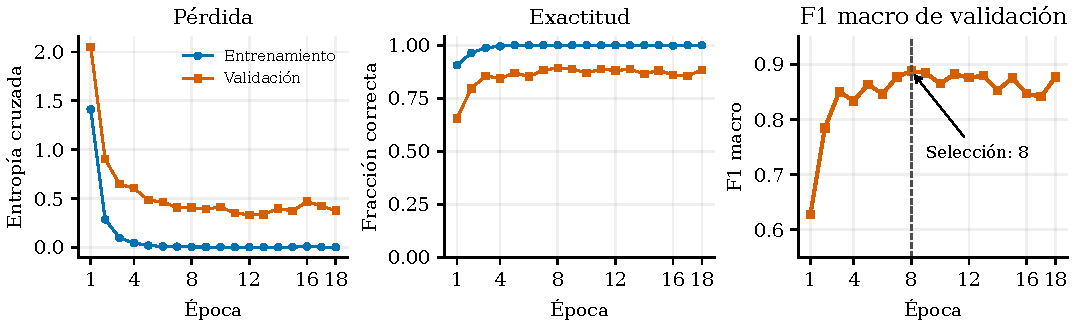
\includegraphics[width=\textwidth]{figuras/curves.pdf}
\caption{Historial guardado de YOLO26m-cls completo, 40 fotos por clase, tasa $10^{-4}$ y semilla 42. Pérdida, exactitud y F1 en paneles separados; línea discontinua en la época seleccionada. Las métricas de entrenamiento se calculan sin aumento después de cada época.}
\label{fig:curves}
\end{figure*}

\subsection{Evaluación del checkpoint oficial}
{\raggedright La selección quedó registrada en Git \artifact{61fe046} antes de la prueba; la fuente de entrenamiento es \artifact{5c213fa} y la de evaluación \artifact{c8b48af}. La corrida ganadora es \artifact{d59207e9411549868004183bbf8ee4cd}, modelo nativo \nolinkurl{models:/m-393ef6ee2c23452197cee6f388941bcf}. \par} En la época 8 su F1 de validación es $0{,}887945$ y su exactitud $0{,}891667$: valores de la semilla 42, distintos de la media usada para elegir la configuración.

{\raggedright La prueba oficial corresponde a la corrida \artifact{8f50ccb1f784460d953fff8fc94ef3f0}.\par} La Tabla~\ref{tab:test} resume 543 aciertos y 57 errores sobre 600 fotografías. Solo se evalúa este checkpoint en prueba; no se presenta una comparación de prueba entre familias ni una media de prueba entre semillas. Las 50 marcas de incertidumbre están incluidas en el denominador. De ellas, 28 son errores y 22 aciertos; entre las 550 restantes hay 29 errores y 521 aciertos. Por tanto, el umbral no identifica todos los errores y también marca predicciones correctas.

\begin{table}[t]\centering\small
\caption{Prueba oficial del checkpoint prefijado de semilla 42.}
\label{tab:test}
\begin{tabular}{lr}\toprule
Medida & Valor\\\midrule
Fotografías / aciertos / errores & 600 / 543 / 57\\
Exactitud & $0{,}9050$\\
F1 macro & $0{,}9043$\\
Entropía cruzada media & $0{,}3424$\\
Puntuaciones $<0{,}50$ incluidas & 50\\\bottomrule
\end{tabular}
\end{table}

\subsection{Errores sistemáticos y efecto documental}
La Fig.~\ref{fig:confusion} muestra las 40 clases con soporte de 15 fotos cada una. La Tabla~\ref{tab:pairs} conserva los cuatro pares empatados con cinco errores al sumar direcciones. Por ejemplo, Chanfainita se propone como Cau Cau cinco veces y no ocurre el error inverso en prueba; Choclo con Queso se propone como Ceviche cinco veces y tampoco ocurre el inverso. La asimetría ayuda a localizar qué clases pierden sensibilidad y cuáles acumulan falsos positivos. No prueba que el modelo use un ingrediente, color o fondo particular. Humitas/Tamales y Rocoto Relleno/Tacu Tacu comparten el mismo máximo y no deben omitirse por un orden arbitrario de clasificación.

\begin{table}[t]\centering\footnotesize
\caption{Todos los pares empatados en el máximo de confusión. A$\to$B indica clase real A propuesta como B.}
\label{tab:pairs}\setlength{\tabcolsep}{4pt}
\begin{tabular}{llrrr}\toprule
Clase A & Clase B & A$\to$B & B$\to$A & Total\\\midrule
Cau Cau & Chanfainita & 0 & 5 & 5\\
Ceviche & Choclo con Queso & 0 & 5 & 5\\
Humitas & Tamales & 5 & 0 & 5\\
Rocoto Relleno & Tacu Tacu & 5 & 0 & 5\\\bottomrule
\end{tabular}
\end{table}

\begin{figure*}[t]\centering
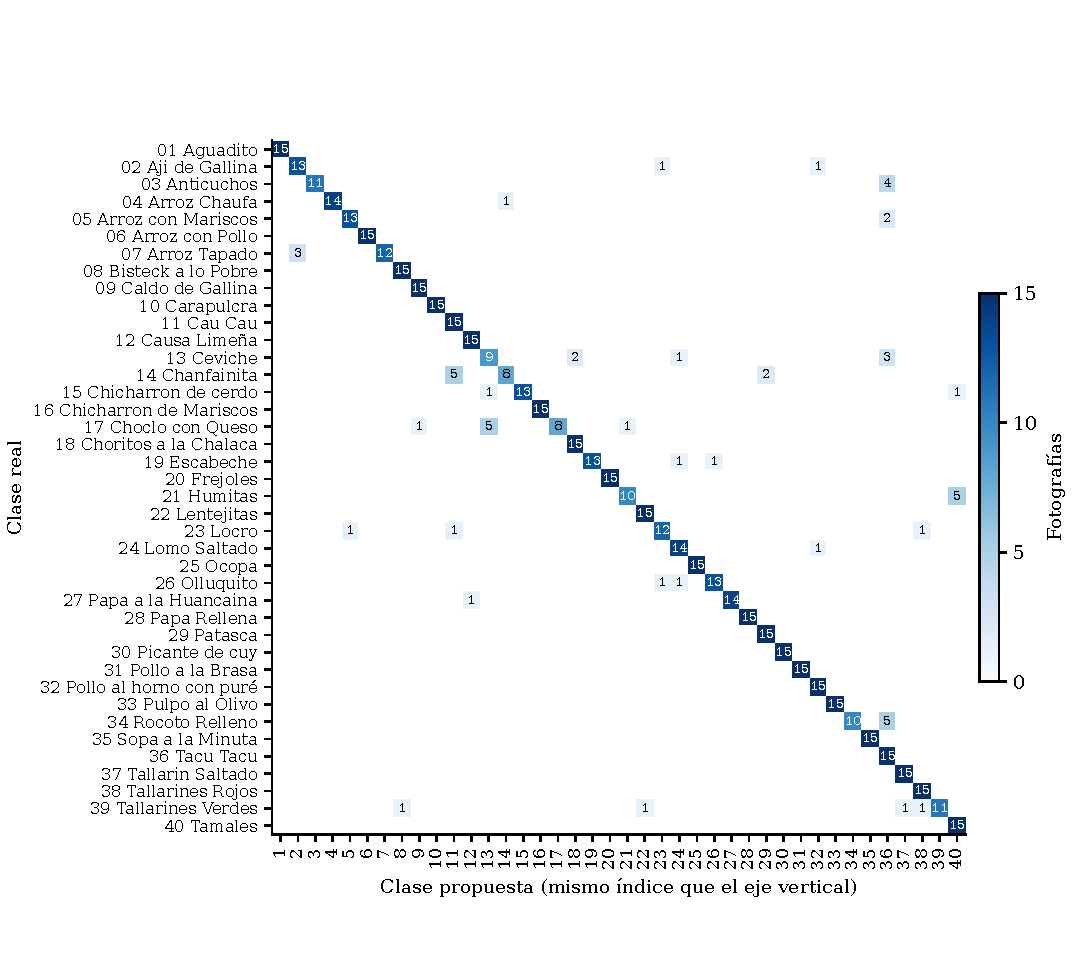
\includegraphics[width=\textwidth]{figuras/confusion.pdf}
\caption{Matriz de confusión reconstruida desde las predicciones guardadas de prueba. Las celdas indican fotografías; blanco representa cero. Los índices horizontales corresponden a los mismos nombres e índices del eje vertical. Filas: clase real; columnas: clase propuesta.}
\label{fig:confusion}
\end{figure*}

El caso de la Fig.~\ref{fig:error} es el primer error, en el orden del manifiesto, cuyas uniones documentales de ingredientes difieren. La imagen de ají de gallina \nolinkurl{72_Aji_de_Gallina.jpg} se clasificó como Locro con $s=0{,}305247$, por lo que se marcó incierta. La Tabla~\ref{tab:recipe} compara las fichas usando la unión de las dos columnas del estudio original: las tablas 1 y 2 de \cite{arzola2025} definen los códigos y su asociación a platos. La consulta equivocada omite de esa unión apio y frutos de cáscara. Esto es una diferencia entre listas de recetas, no una omisión visualmente demostrada de ingredientes presentes en la fotografía.

\begin{figure}[t]\centering
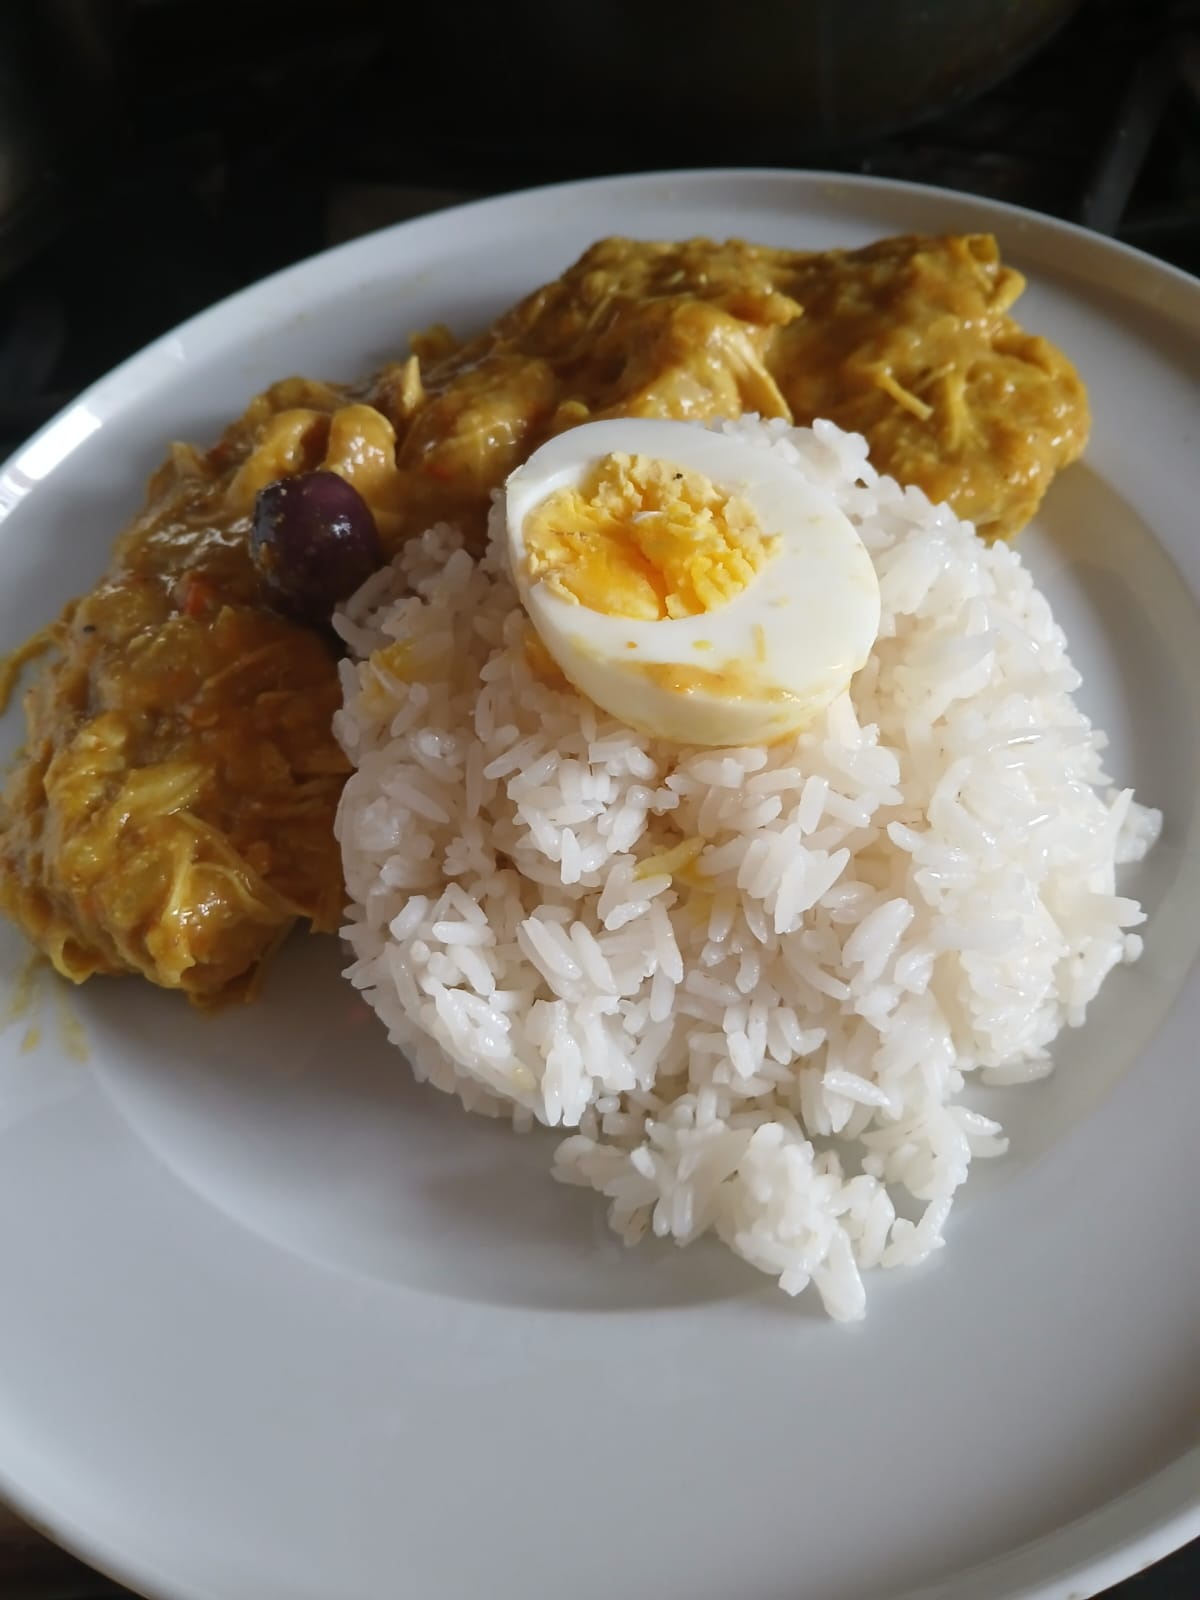
\includegraphics[width=0.78\columnwidth,height=4.1cm,keepaspectratio]{figuras/error.jpg}
\caption{Error real: ají de gallina propuesto como locro; puntuación $0{,}305247$, incierto. Foto de Arzola, Canchari y Escobedo, PeruFoodNet V3, CC BY 4.0 \cite{perufoodnetv3}; copia de la evidencia guardada, sin alteración de contenido.}
\label{fig:error}
\end{figure}

\begin{table}[t]\centering\footnotesize
\caption{Unión documental de códigos de receta para el caso de error. AI001: apio; AI004: huevos; AI007: leche; AI010: frutos de cáscara. Fuente: tablas 1 y 2 de \cite{arzola2025}.}
\label{tab:recipe}
\begin{tabular}{lp{5.2cm}}\toprule
Ficha & Códigos de posibles ingredientes\\\midrule
Ají de gallina & AI001, AI004, AI007, AI010\\
Locro & AI004, AI007\\
Diferencia & AI001 y AI010 solo en la ficha de ají de gallina\\\bottomrule
\end{tabular}
\end{table}

\subsection{Costo computacional y ejecución}
La Tabla~\ref{tab:cost} separa las mediciones de tiempo. La campaña final consumió 55 min 43 s de reloj; la suma de las duraciones de las 32 corridas fue 3.189,05 s, aproximadamente 0,886 h en el equipo con RTX 5090. Esta aproximación de horas de ejecución con GPU incluye carga, preparación, entrenamiento, validación por época y registro/recuperación del modelo, hasta antes de la última subida de artefactos. No mide ocupación continua del procesador gráfico ni tiempo puro de kernels. Tampoco suma los intentos preliminares y controles al costo de la matriz final. No se midieron electricidad, emisiones ni costo monetario.

\begin{table}[t]\centering\footnotesize
\caption{Recursos y tiempos con alcances distintos.}
\label{tab:cost}
\begin{tabular}{lp{4.9cm}}\toprule
Medida & Valor y alcance\\\midrule
Hardware & RTX 5090, aproximadamente 32 GB\\
Campaña final & 55 min 43 s de reloj\\
Suma de 32 corridas & 53 min 9 s $\simeq0{,}886$ h; preparación y registro incluidos\\
Prueba oficial & 11,03 s; carga, preparación y una pasada; excluye figuras, MLflow y benchmark\\
Latencia de red & 2,873 ms; lote 1 sintético de $224\times224$, 30 calentamientos y 200 iteraciones\\
Checkpoint final & 41.802.085 bytes; 41,80 MB decimales, aproximadamente 39,87 MiB\\\bottomrule
\end{tabular}
\end{table}

La latencia de red excluye lectura y preprocesamiento: no es latencia de extremo a extremo ni evidencia de rendimiento en CPU o teléfono. El checkpoint de demostración se carga sin el dataset completo, los pesos iniciales ni MLflow. Hay dos notebooks, uno de exploración y otro de inferencia de una imagen; entrenamiento y evaluación están en \artifact{src/}. La ejecución fue verificada localmente. Colab y sus enlaces de descarga están preparados, pero no se ejecutaron ni se probaron sus descargas.

\section{Discusión}
\subsection{Qué respalda la comparación}
La ablación a tasa fija respalda que ajustar el extractor es útil en estas condiciones. Una interpretación compatible con la transferencia es que la representación inicial no separa completamente los platos y que adaptarla mejora la frontera de decisión; la ablación mide el resultado, no demuestra qué filtros o atributos causan la mejora. El aumento de presupuesto también acompaña mejores medias en todas las condiciones seleccionadas. Como los archivos están ordenados y no se muestrearon raciones independientes, esa observación no se extrapola a una ley general de eficiencia de datos.

El F1 de prueba supera ligeramente al F1 de validación de la semilla 42. Esto no demuestra mejor generalización: son conjuntos distintos de fotografías, pequeños por clase, y posiblemente dependientes. No se ajustaron hiperparámetros ni umbrales a partir de prueba. La comparación entre familias se hace en validación y está condicionada por la búsqueda de tasas; no puede presentarse como una victoria estadística confirmada.

\subsection{Validez, sesgos y límites}
El límite principal es la unidad de partición. Se respetó el reparto solicitado de números de archivo, pero no se agruparon las vistas por ración. Una misma preparación podría estar representada en entrenamiento, validación y prueba. Por ello, la independencia por ración y la ausencia de fuga por contenido no están acreditadas. El resultado de 0,9043 no estima de manera fiable el rendimiento sobre raciones, restaurantes o fotografías externas nuevas. Una evaluación con separación por ración sería necesaria antes de sostener esa conclusión.

El balance de clases no garantiza diversidad de recetas, restaurantes, dispositivos o contextos. La reducción directa a una imagen cuadrada puede deformar relaciones geométricas. Con pocos ejemplos por clase y solo tres semillas no se caracteriza la variabilidad entre particiones ni el efecto de todas las decisiones de preprocesamiento. No se ensayaron otras familias, tasas adicionales, entrenamiento desde cero o calibración; tampoco se evaluaron escenas con varios platos o clases desconocidas. La selección identifica una configuración dentro del alcance fijado, no una solución universal.

\subsection{Impacto y uso responsable}
Una aplicación informativa puede facilitar la consulta de platos y recetas, siempre que muestre su incertidumbre y la procedencia documental. Sin embargo, ni una clasificación correcta prueba los ingredientes de una preparación concreta, ni una lista sin un código prueba ausencia de ese ingrediente. Las recetas varían y el contacto cruzado no se observa en esta tarea. La ficha debe apoyar preguntas al establecimiento sobre preparación e ingredientes; no acredita seguridad alimentaria ni sustituye esa confirmación.

El error de ají de gallina ilustra una consecuencia verificable: cambiar el nombre propuesto cambia la lista consultada. La puntuación baja permite señalar incertidumbre en ese caso, pero los 29 errores con puntuación al menos 0,50 muestran el límite del umbral. No se dispone de calibración ni validación de detección fuera de distribución. La difusión de los resultados debe conservar esas restricciones y la atribución de las imágenes reutilizadas.

\section{Conclusiones y trabajo futuro}
En la partición secuencial estudiada, el ajuste completo mejora el F1 de validación frente a la última capa lineal en las ocho comparaciones de tasa fija y semilla 42. La matriz de 32 corridas selecciona YOLO26m-cls completo con 40 imágenes por clase y tasa $10^{-4}$ por su media de validación. La diferencia respecto a ResNet-18 completo no establece superioridad estadística. El checkpoint prefijado de semilla 42 obtiene 543 aciertos de 600 y F1 macro 0,9043; ese resultado describe esta partición y queda limitado por la posible correlación de vistas entre conjuntos.

El trabajo futuro prioritario es identificar raciones o sesiones de captura y reconstruir particiones agrupadas, seguidas de una prueba externa por restaurante y dispositivo. Después corresponde ampliar semillas y particiones para comparar familias, estudiar calibración con datos independientes y evaluar clases desconocidas y escenas con varios platos. La ficha de recetas requeriría una evaluación documental y de interacción propia; el experimento actual no valida detección de ingredientes ni ausencia de alérgenos o contacto cruzado.

\section*{Contribuciones}
La Tabla~\ref{tab:contributions} presenta las tareas efectivamente realizadas y confirmadas para cada integrante. El grupo informó autorización docente para cinco integrantes.

\begin{table}[ht]\centering\footnotesize
\caption{Contribuciones individuales confirmadas.}
\label{tab:contributions}
\begin{tabular}{>{\raggedright\arraybackslash\hyphenpenalty=10000}p{3.5cm}p{4cm}}\toprule
Integrante & Tareas reales\\\midrule
Josué Chilón Cruzado & Preparación y exploración de datos y verificación de partición\\
Miguel Ángel Concepción Tiza & Modelos de transferencia y entrenamiento\\
Enzo Israel Neyra Dianderas & Matriz experimental, seguimiento MLflow y selección por validación\\
Omar Salvador Tello Guerra & Evaluación en prueba, análisis de errores y limitaciones\\
Alexander Vladimir Paco Cornejo & Demostración, ficha de ingredientes y reproducción de resultados\\\bottomrule
\end{tabular}
\end{table}

\section*{Disponibilidad y uso de herramientas de IA}
La carpeta hermana \textit{3.3 Código} contiene el código y las evidencias de R03.1; allí \artifact{results/winner.json} identifica la selección y las rutas locales del checkpoint. La entrega se identifica como \texttt{v1.0-final} en el repositorio del curso \cite{entrega2026}. Sus activos son \nolinkurl{Equipo3_Codigo.zip}, con el proyecto y sus evidencias, y \nolinkurl{perufoodnet_best.pt}, con los pesos de la demostración. Esta comprueba la integridad de los pesos.

Se utilizó OpenAI Codex con modelos GPT-6.1 Terra, GPT-6.1 Sol y GPT-6 Astra como apoyo para preparar y depurar código, organizar experimentos, revisar evidencias y elaborar y revisar documentación. GPT-6.1 Sol asistió en la redacción, las figuras derivadas de archivos guardados y la compilación de este artículo. Las cifras proceden de ejecuciones locales registradas y de sus CSV y JSON; no son resultados generados por un modelo de lenguaje. Esta declaración describe el uso de herramientas y no asigna tareas humanas ni autoría a los asistentes.

\bibliographystyle{IEEEtran}
\bibliography{references}
\end{document}
